\begin{enumerate}[label=\thesubsection.\arabic*.,ref=\thesubsection.\theenumi]
\numberwithin{equation}{enumi}

\item In the block diagram Fig.\ref{fig:ee18btech11029}  
\begin{align}
G\brak{s} = \frac{K}{\brak{s+4}\brak{s+5}}
\label{ee18btech11034_Gs}
\end{align}
\begin{figure}[!ht]
    \begin{center}
		\resizebox{\columnwidth}{!}{%\begin{enumerate}[label=\thesubsection.\arabic*.,ref=\thesubsection.\theenumi]
%\numberwithin{equation}{enumi}
\item
Sketch the Polar Plot of
\begin{align}
G\brak{s} = \frac{\brak{1+\frac{s}{29}}\brak{1+0.0025s}}{\brak{s^{3}}\brak{1+0.005s}\brak{1+0.001s}}
\end{align}

\solution 
%
The following code generates the polar plot in Fig.   \ref{fig:ee18btech11029}

\begin{lstlisting}
codes/ee18btech11029.py
\end{lstlisting}

\begin{figure}[!h]
\centering
  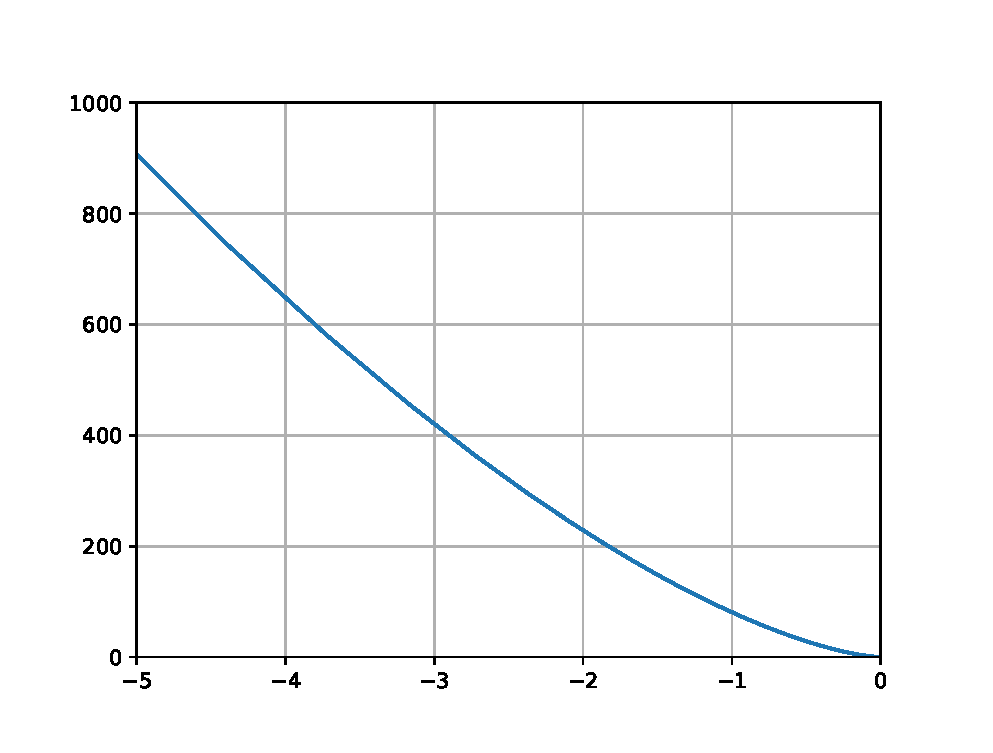
\includegraphics[width=\columnwidth]{./figs/ee18btech11029.eps}
  \caption{}
  \label{fig:ee18btech11029}
\end{figure}

\begin{itemize}
    \item The polar plots use open loop transfer function to determine the stability and hence reference point is shifted to \brak{-1,0}
    \item If \brak{–1,0} is left of the polar plot or \brak{–1,0} is not enclosed, then it is stable
    \item If \brak{–1,0} is on right side of the polar plot or \brak{–1,0} is enclosed by polar plot then it is unstable. 
    \item If \brak{–1,0} is on the polar plot then it is marginally stable
    
\end{itemize}

In Fig.   \ref{fig:ee18btech11029},  \brak{-1,0} is on the polar plot so the system is marginally stable.
   
%\end{enumerate}
}
	\end{center}
\caption{}
\label{fig:ee18btech11029}
\end{figure}
\item Find the range of K for stability by Nyquist criterion

\solution
\begin{figure}[!h]
    \begin{center}
		\resizebox{\columnwidth}{!}{\tikzset{
        block/.style = {draw, rectangle,
            minimum height=1cm,
            minimum width=2cm},
        input/.style = {coordinate,node distance=1cm},
        output/.style = {coordinate,node distance=4cm},
        arrow/.style={draw, -latex,node distance=2cm},
        pinstyle/.style = {pin edge={latex-, black,node distance=2cm}},
        sum/.style = {draw, circle, node distance=1cm},
}

\begin{tikzpicture}[node distance=2.5cm,auto,>=latex']
  \node [input, name=input] {};
  \node [sum, right of=input] (sum) {};
  \node [block, right of = sum] (block1) {$\frac{G(s)}{1+G(s)}$};
  \node [block, right of = block1] (block2) {$\frac{G(s)}{1+G(s)}$};
  \node [output, right of= block2] (output) {};
  \draw [->] (input) -- node {$R(s)\ +$} (sum);
  \draw [->] (sum) -- node {} (block1);
  \draw [->] (block1) -- node {} (block2);
  \draw [->] (block2) -- node [name =y] {$Y(s)$} (output);
  \draw [->] (y) -- ++ (0,-2) -| node [pos=0.99] {$+$} (sum);
\end{tikzpicture}
}
	\end{center}
\caption{}
\label{fig:ee18btech11029_1}
\end{figure}


The open loop transfer function from Fig.\ref{fig:ee18btech11029_1}

\begin{align}
    T\brak{s} =\brak{\frac{\frac{K}{\brak{s+4}\brak{s+5}}}{1+\frac{K}{\brak{s+4}\brak{s+5}}}}^2 
\end{align}


\begin{align}
    T\brak{\j\omega} =\brak{\frac{\frac{K}{\brak{\j\omega+4}\brak{\j\omega+5}}}{1+\frac{K}{\brak{\j\omega+4}\brak{\j\omega+5}}}}^2 
\end{align}




\begin{itemize}
    \item Since it is connected in positive feedback the transfer function cuts at \brak{1,\j0} 
\end{itemize}

\begin{align}
    \implies  \text{Re} \cbrak{T\brak{\j\omega}} &= 1\\
      \implies  \text{Im} \cbrak{T\brak{\j \omega}} &= 0
     \label{eq:ee18btech11029_eq_Re}
\end{align}


\begin{align}
    \brak{\frac{\frac{K}{\brak{\j\omega+4}\brak{\j\omega+5}}}{1+\frac{K}{\brak{\j\omega+4}\brak{\j\omega+5}}}}^2 &= 1+\j0
\end{align}

\begin{align}
    \brak{\j\omega+4}\brak{\j\omega+5}+2K &=0
\end{align}

\begin{align}
    -\omega^2 + 9\j\omega +20+2K &=0 
\end{align}
\\
From  \eqref{eq:ee18btech11029_eq_Re}

\begin{align}
    20 + 2K &= 0\\
    \implies K=-10
\end{align}
The minimum value of stability for the system to be stable is
\begin{align}
    K_{min} > -10
\end{align}
The range of K for which the system is stable is 
\begin{align}
    -10 < K < \infty
\end{align}


\item From the table.\ref{table:ee18btech11029_table1}, 
Stability criterion for K is N+P=Z


\begin{table}[!h]
\centering
%%%%%%%%%%%%%%%%%%%%%%%%%%%%%%%%%%%%%%%%%%%%%%%%%%%%%%%%%%%%%%%%%%%%%%
%%                                                                  %%
%%  This is the header of a LaTeX2e file exported from Gnumeric.    %%
%%                                                                  %%
%%  This file can be compiled as it stands or included in another   %%
%%  LaTeX document. The table is based on the longtable package so  %%
%%  the longtable options (headers, footers...) can be set in the   %%
%%  preamble section below (see PRAMBLE).                           %%
%%                                                                  %%
%%  To include the file in another, the following two lines must be %%
%%  in the including file:                                          %%
%%        \def\inputGnumericTable{}                                 %%
%%  at the beginning of the file and:                               %%
%%        \input{name-of-this-file.tex}                             %%
%%  where the table is to be placed. Note also that the including   %%
%%  file must use the following packages for the table to be        %%
%%  rendered correctly:                                             %%
%%    \usepackage[latin1]{inputenc}                                 %%
%%    \usepackage{color}                                            %%
%%    \usepackage{array}                                            %%
%%    \usepackage{longtable}                                        %%
%%    \usepackage{calc}                                             %%
%%    \usepackage{multirow}                                         %%
%%    \usepackage{hhline}                                           %%
%%    \usepackage{ifthen}                                           %%
%%  optionally (for landscape tables embedded in another document): %%
%%    \usepackage{lscape}                                           %%
%%                                                                  %%
%%%%%%%%%%%%%%%%%%%%%%%%%%%%%%%%%%%%%%%%%%%%%%%%%%%%%%%%%%%%%%%%%%%%%%



%%  This section checks if we are begin input into another file or  %%
%%  the file will be compiled alone. First use a macro taken from   %%
%%  the TeXbook ex 7.7 (suggestion of Han-Wen Nienhuys).            %%
\def\ifundefined#1{\expandafter\ifx\csname#1\endcsname\relax}


%%  Check for the \def token for inputed files. If it is not        %%
%%  defined, the file will be processed as a standalone and the     %%
%%  preamble will be used.                                          %%
\ifundefined{inputGnumericTable}

%%  We must be able to close or not the document at the end.        %%
	\def\gnumericTableEnd{\end{document}}


%%%%%%%%%%%%%%%%%%%%%%%%%%%%%%%%%%%%%%%%%%%%%%%%%%%%%%%%%%%%%%%%%%%%%%
%%                                                                  %%
%%  This is the PREAMBLE. Change these values to get the right      %%
%%  paper size and other niceties.                                  %%
%%                                                                  %%
%%%%%%%%%%%%%%%%%%%%%%%%%%%%%%%%%%%%%%%%%%%%%%%%%%%%%%%%%%%%%%%%%%%%%%

	\documentclass[12pt%
			  %,landscape%
                    ]{report}
       \usepackage[latin1]{inputenc}
       \usepackage{fullpage}
       \usepackage{color}
       \usepackage{array}
       \usepackage{longtable}
       \usepackage{calc}
       \usepackage{multirow}
       \usepackage{hhline}
       \usepackage{ifthen}

	\begin{document}


%%  End of the preamble for the standalone. The next section is for %%
%%  documents which are included into other LaTeX2e files.          %%
\else

%%  We are not a stand alone document. For a regular table, we will %%
%%  have no preamble and only define the closing to mean nothing.   %%
    \def\gnumericTableEnd{}

%%  If we want landscape mode in an embedded document, comment out  %%
%%  the line above and uncomment the two below. The table will      %%
%%  begin on a new page and run in landscape mode.                  %%
%       \def\gnumericTableEnd{\end{landscape}}
%       \begin{landscape}


%%  End of the else clause for this file being \input.              %%
\fi

%%%%%%%%%%%%%%%%%%%%%%%%%%%%%%%%%%%%%%%%%%%%%%%%%%%%%%%%%%%%%%%%%%%%%%
%%                                                                  %%
%%  The rest is the gnumeric table, except for the closing          %%
%%  statement. Changes below will alter the table's appearance.     %%
%%                                                                  %%
%%%%%%%%%%%%%%%%%%%%%%%%%%%%%%%%%%%%%%%%%%%%%%%%%%%%%%%%%%%%%%%%%%%%%%

\providecommand{\gnumericmathit}[1]{#1} 
%%  Uncomment the next line if you would like your numbers to be in %%
%%  italics if they are italizised in the gnumeric table.           %%
%\renewcommand{\gnumericmathit}[1]{\mathit{#1}}
\providecommand{\gnumericPB}[1]%
{\let\gnumericTemp=\\#1\let\\=\gnumericTemp\hspace{0pt}}
 \ifundefined{gnumericTableWidthDefined}
        \newlength{\gnumericTableWidth}
        \newlength{\gnumericTableWidthComplete}
        \newlength{\gnumericMultiRowLength}
        \global\def\gnumericTableWidthDefined{}
 \fi
%% The following setting protects this code from babel shorthands.  %%
 \ifthenelse{\isundefined{\languageshorthands}}{}{\languageshorthands{english}}
%%  The default table format retains the relative column widths of  %%
%%  gnumeric. They can easily be changed to c, r or l. In that case %%
%%  you may want to comment out the next line and uncomment the one %%
%%  thereafter                                                      %%
\providecommand\gnumbox{\makebox[0pt]}
%%\providecommand\gnumbox[1][]{\makebox}

%% to adjust positions in multirow situations                       %%
\setlength{\bigstrutjot}{\jot}
\setlength{\extrarowheight}{\doublerulesep}

%%  The \setlongtables command keeps column widths the same across  %%
%%  pages. Simply comment out next line for varying column widths.  %%
\setlongtables

\setlength\gnumericTableWidth{%
	25pt+%
	25pt+%
	25pt+%
	25pt+%
	50pt+%
0pt}
\def\gumericNumCols{5}
\setlength\gnumericTableWidthComplete{\gnumericTableWidth+%
         \tabcolsep*\gumericNumCols*2+\arrayrulewidth*\gumericNumCols}
\ifthenelse{\lengthtest{\gnumericTableWidthComplete > \linewidth}}%
         {\def\gnumericScale{\ratio{\linewidth-%
                        \tabcolsep*\gumericNumCols*2-%
                        \arrayrulewidth*\gumericNumCols}%
{\gnumericTableWidth}}}%
{\def\gnumericScale{1}}

%%%%%%%%%%%%%%%%%%%%%%%%%%%%%%%%%%%%%%%%%%%%%%%%%%%%%%%%%%%%%%%%%%%%%%
%%                                                                  %%
%% The following are the widths of the various columns. We are      %%
%% defining them here because then they are easier to change.       %%
%% Depending on the cell formats we may use them more than once.    %%
%%                                                                  %%
%%%%%%%%%%%%%%%%%%%%%%%%%%%%%%%%%%%%%%%%%%%%%%%%%%%%%%%%%%%%%%%%%%%%%%

\ifthenelse{\isundefined{\gnumericColA}}{\newlength{\gnumericColA}}{}\settowidth{\gnumericColA}{\begin{tabular}{@{}p{25pt*\gnumericScale}@{}}x\end{tabular}}
\ifthenelse{\isundefined{\gnumericColB}}{\newlength{\gnumericColB}}{}\settowidth{\gnumericColB}{\begin{tabular}{@{}p{25pt*\gnumericScale}@{}}x\end{tabular}}
\ifthenelse{\isundefined{\gnumericColC}}{\newlength{\gnumericColC}}{}\settowidth{\gnumericColC}{\begin{tabular}{@{}p{25pt*\gnumericScale}@{}}x\end{tabular}}
\ifthenelse{\isundefined{\gnumericColD}}{\newlength{\gnumericColD}}{}\settowidth{\gnumericColD}{\begin{tabular}{@{}p{25pt*\gnumericScale}@{}}x\end{tabular}}
\ifthenelse{\isundefined{\gnumericColE}}{\newlength{\gnumericColE}}{}\settowidth{\gnumericColE}{\begin{tabular}{@{}p{50pt*\gnumericScale}@{}}x\end{tabular}}

\begin{tabular}[c]{%
	b{\gnumericColA}%
	b{\gnumericColB}%
	b{\gnumericColC}%
	b{\gnumericColD}%
	b{\gnumericColE}%
	}

%%%%%%%%%%%%%%%%%%%%%%%%%%%%%%%%%%%%%%%%%%%%%%%%%%%%%%%%%%%%%%%%%%%%%%
%%  The longtable options. (Caption, headers... see Goosens, p.124) %%
%	\caption{The Table Caption.}             \\	%
% \hline	% Across the top of the table.
%%  The rest of these options are table rows which are placed on    %%
%%  the first, last or every page. Use \multicolumn if you want.    %%

%%  Header for the first page.                                      %%
%	\multicolumn{3}{c}{The First Header} \\ \hline 
%	\multicolumn{1}{c}{colTag}	%Column 1
%	&\multicolumn{1}{c}{colTag}	%Column 2
%	&\multicolumn{1}{c}{colTag}	\\ \hline %Last column
%	\endfirsthead

%%  The running header definition.                                  %%
%	\hline
%	\multicolumn{3}{l}{\ldots\small\slshape continued} \\ \hline
%	\multicolumn{1}{c}{colTag}	%Column 1
%	&\multicolumn{1}{c}{colTag}	%Column 2
%	&\multicolumn{1}{c}{colTag}	\\ \hline %Last column
%	\endhead

%%  The running footer definition.                                  %%
%	\hline
%	\multicolumn{3}{r}{\small\slshape continued\ldots} \\
%	\endfoot

%%  The ending footer definition.                                   %%
%	\multicolumn{3}{c}{That's all folks} \\ \hline 
%	\endlastfoot
%%%%%%%%%%%%%%%%%%%%%%%%%%%%%%%%%%%%%%%%%%%%%%%%%%%%%%%%%%%%%%%%%%%%%%

\hhline{|-|-|-|-|-}
	 \multicolumn{1}{|p{\gnumericColA}|}%
	{\gnumericPB{\centering}\textbf{K}}
	&\multicolumn{1}{p{\gnumericColB}|}%
	{\gnumericPB{\centering}\textbf{P}}
	&\multicolumn{1}{p{\gnumericColC}|}%
	{\gnumericPB{\centering}\textbf{N}}
	&\multicolumn{1}{p{\gnumericColD}|}%
	{\gnumericPB{\centering}\textbf{Z}}
	&\multicolumn{1}{p{\gnumericColE}|}%
	{\gnumericPB{\raggedright}\textbf{Description}}
	
\\
\hhline{|-----|}
	 \multicolumn{1}{|p{\gnumericColA}|}%
	{\gnumericPB{\centering}-10}
	&\multicolumn{1}{p{\gnumericColB}|}%
	{\gnumericPB{\centering}0}
	&\multicolumn{1}{p{\gnumericColC}|}%
	{\gnumericPB{\centering}0}
	&\multicolumn{1}{p{\gnumericColD}|}%
	{\gnumericPB{\centering}0}
	&\multicolumn{1}{p{\gnumericColE}|}%
	{\gnumericPB{\raggedright}System is marginally stable}
\\
\hhline{|-----|}
	 \multicolumn{1}{|p{\gnumericColA}|}%
	{\gnumericPB{\centering}-9}
	&\multicolumn{1}{p{\gnumericColB}|}%
	{\gnumericPB{\centering}0}
	&\multicolumn{1}{p{\gnumericColC}|}%
	{\gnumericPB{\centering}0}
	&\multicolumn{1}{p{\gnumericColD}|}%
	{\gnumericPB{\centering}0}
	&\multicolumn{1}{p{\gnumericColE}|}%
	{\gnumericPB{\raggedright}System is stable}
\\
\hhline{|-----|}
	 \multicolumn{1}{|p{\gnumericColA}|}%
	{\gnumericPB{\centering}-11}
	&\multicolumn{1}{p{\gnumericColB}|}%
	{\gnumericPB{\centering}0}
	&\multicolumn{1}{p{\gnumericColC}|}%
	{\gnumericPB{\centering}1}
	&\multicolumn{1}{p{\gnumericColD}|}%
	{\gnumericPB{\centering}1}
	&\multicolumn{1}{p{\gnumericColE}|}%
	{\gnumericPB{\raggedright}System is unstable}
\\
\hhline{|-|-|-|-|-|}
\end{tabular}

\ifthenelse{\isundefined{\languageshorthands}}{}{\languageshorthands{\languagename}}
\gnumericTableEnd

\caption{}
\label{table:ee18btech11029_table1}
\end{table}


\item Verify the Nyquist plots by
\begin{lstlisting}
codes/ee18btech11029_1.py
\end{lstlisting}


\begin{figure}[h!]
\centering
  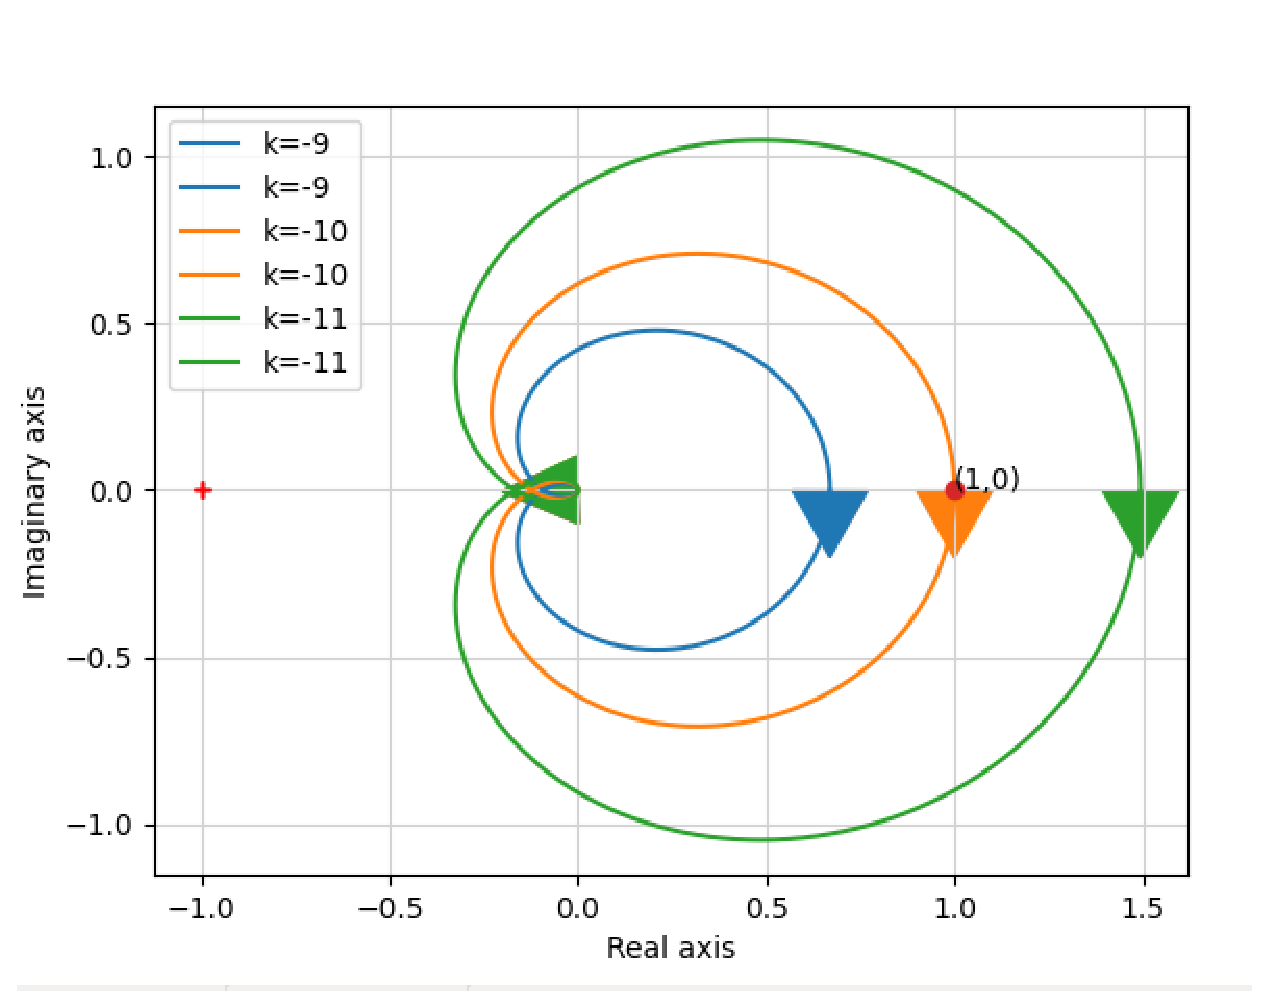
\includegraphics[width=\columnwidth]{./figs/ee18btech11029/Nyquist.eps}
  \caption{Nyquist Plot}
  \label{fig:ee18btech11029_2}
\end{figure}





\item Verify the result using Routh-Hurwitz criterion

\solution The characteristic equation is 
\begin{align}
    1-T\brak{s} &=0\\
    1-\brak{\frac{\frac{K}{\brak{s+4}\brak{s+5}}}{1+\frac{K}{\brak{s+4}\brak{s+5}}}}^2 &=0\\
    1+2\brak{\frac{K}{\brak{s+4}\brak{s+5}}}&=0\\
    s^2+9s+20+2K &= 0
\end{align}

\begin{align}
\mydet{s^2\\s^1\\s^0}
\mydet{1 & 20+2K \\ 9 & 0 \\ 20+2K & 0}
\end{align}
For a system to be stable it should not have any sign changes
\begin{align}
    20+2K >0
\end{align}
This is valid for all positive values of K but the minimum value of K is
\begin{align}
    K>-10
\end{align}
So the range of K for stability is 
\begin{align}
    -10<K<\infty
\end{align}

\item Verify the result by
\begin{lstlisting}
codes/ee18btech11029_2.py
\end{lstlisting}







\end{enumerate}
